\documentclass[main]{subfiles}
\begin{document}

%@@@@@@@@@@@@@@@@@@@@@@@@@@@@@@
% Main Topics: graphs and TU matrices, max-flow min-cut
% Applications of Total Unimodularity - 16.11.2017
% Joe covered Weismantell in this lecture
% author: Vanessa Leite

\section{Applications of Total Unimodularity}

\paragraph{A important reminder:}
Theorem: $A \in \{0, \pm 1\}^{m \times n}$ is TU iff $\forall J \subseteq [n]$
(or $J \subseteq [m]$ because $A^T$ is also TU) $\exists$ partition $J = J_1
\cup J_2$ such that $\sum_{j \in J_1} A_{ij} - \sum_{j \in J_2} A_{ij} \in \{0,
\pm 1\}$ iff $\max \{c^T x \mid Ax \leq b\}$ has an \textbf{integral} optimal
solution for every $b \in \Z^n$, wherever an optimal solution exists, iff $A^T$
is TU.

\paragraph{Definition - Digraph}
Let $V$ be a finite set and $A \subseteq V \times V$. Then $D=(V,A)$ is a
digraph (directed graph).

\paragraph{Definition - Node-arc incidence matrix}
The node-arc incidence matrix of $D=(V,A)$ is the matrix
$M \in \{0, \pm1\}^{\abs{V} \times \abs{A}}$, where $M_{ia} = 
\left\{
  \begin{array}{ll}
    1 & \text{if } (i,j) = a \\
    -1 & \text{if } (j,i) = a \\
    0 & \text{else}
  \end{array}
\right.$

\paragraph{Definition}
Let $w \subseteq V$.\\
$\delta^+(w) = \{(i,j) \in A, i \in w, j \notin w \}$.\\
$\delta^-(w) = \{(i,j) \in A, i \notin w, j \in w \}$.\\
\subparagraph{Example:}
\begin{figure}[!h]
  \label{fig:projection}
  \centering
    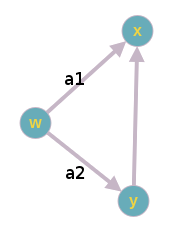
\includegraphics[width=0.3\textwidth]{imgs/graph-definition.png}
\end{figure}

$\delta^+(w) = \{a1,a2\}$.\\
$\delta^-(w) = \emptyset$.\\

\paragraph{Definition - Node-edge incidence matrix}
The node-edge incidence matrix of an undirected graph $G=(V,E)$ is
$M \in \{0,1\}^{\abs{V} \times \abs{E}}$, where $M_{ve} = 
\left\{
  \begin{array}{ll}
    1 & \text{if } e = (v,w)\\
    0 & \text{else}
  \end{array}
\right.$

\paragraph{Theorem: The following matrices are TU:}
\begin{enumerate}
\item The node-arc incidence matrix of a digraph
\item The node-edge incidence matrix of a bipartite undirected graph
\item An interval matrix, i.e, a $\{0,1\}$ matrix where in each row, the $1$'s
are consecutives.
\end{enumerate}

\subparagraph{Proof:}
\begin{enumerate}
\item Let $M$ be a node-arc incidence matrix of a digraph $D=(V,A)$. Every
column of $M$ has one $1$'s and one $-1$'s. Let $J \subseteq [\abs{V}]$ be a
subset of the rows.
Let $J_1 = J$ and $J_2 = \emptyset$.
Thus, $\sum_{i \in J_1} M_{ij} - \underbrace{\sum_{i \in J_2} M_{ij}}_{=0}
= \sum_{i \in J_1} M_{ij} \in \{0, \pm 1\}^{\abs{A}}$.
\item Let $M$ be a node-edge incidence matrix of a bipartite graph $G=(V,E)$.
Every column of $M$ has two $1$'s. Let $J \subseteq [\abs{V}]$ be a subset
of the rows.
Since $G$ is bipartite, $V = V_1 \cup V_2$. Let $J_1 = J \cap V_1$ and
$J_2 = J \cap V_2$.
Thus, $\sum_{i \in J_1} M_{ij} - \sum_{i \in J_2} M_{ij}
\in \{0, \pm 1\}^{\abs{A}}$.
\end{enumerate}


\paragraph{Maximum stable set problem}

\end{document}
